\documentclass[12pt]{article}
\usepackage[utf8]{inputenc}
\usepackage{amsmath}
\usepackage{csquotes}
\usepackage[ruled,vlined]{algorithm2e}
\usepackage{amssymb}
\usepackage{parskip}
\usepackage{graphicx}
\usepackage{epstopdf}
\usepackage{subcaption}
\usepackage{listings}
\usepackage{url}
\usepackage{cite}
\usepackage{caption}
\usepackage{mathtools}
\usepackage{physics}
\usepackage{bm}
\usepackage{float}
\usepackage{fp}
\usepackage{amssymb}
\usepackage{listings}
\usepackage{pdfpages}
\DeclareMathOperator{\E}{\mathbb{E}}
\DeclareMathOperator{\Var}{\mathbb{V}}
\DeclareMathOperator{\Cov}{\mathbb{C}\text{ov}}
\usepackage{graphicx}
\usepackage{subcaption}
\usepackage{mwe}
\renewcommand{\vec}[1]{\boldsymbol{#1}} % Uncomment for BOLD vectors


% Default fixed font does not support bold face
\DeclareFixedFont{\ttb}{T1}{txtt}{bx}{n}{12} % for bold
\DeclareFixedFont{\ttm}{T1}{txtt}{m}{n}{12}  % for normal

% Custom colors
\usepackage{color}
\definecolor{deepblue}{rgb}{0,0,0.5}
\definecolor{deepred}{rgb}{0.6,0,0}
\definecolor{deepgreen}{rgb}{0,0.5,0}

\usepackage{listings}

% Python style for highlighting
\newcommand\pythonstyle{\lstset{
language=Python,
basicstyle=\ttm,
otherkeywords={self},             % Add keywords here
keywordstyle=\ttb\color{deepblue},
emph={MyClass,__init__},          % Custom highlighting
emphstyle=\ttb\color{deepred},    % Custom highlighting style
stringstyle=\color{deepgreen},
frame=tb,                         % Any extra options here
showstringspaces=false            % 
}}


% Python environment
\lstnewenvironment{python}[1][]
{
\pythonstyle
\lstset{#1}
}
{}

% Python for external files
\newcommand\pythonexternal[2][]{{
\pythonstyle
\lstinputlisting[#1]{#2}}}

% Python for inline
\newcommand\pythoninline[1]{{\pythonstyle\lstinline!#1!}}





\usepackage{times}



\usepackage{geometry}
\usepackage[normalem]{ulem}
\useunder{\uline}{\ul}{}
\linespread{1.5}

%Includes "References" in the table of contents
\usepackage[nottoc]{tocbibind}




\geometry{a4paper,left=3cm,right=3cm,top=2cm,bottom=3cm}
% head
\topskip=1cm
\usepackage{fancyhdr}
\pagestyle{fancy}
\lhead{
\includegraphics[scale=0.5]{figures/dtu_logo.pdf}} 

\chead{}
\rhead{\bfseries 02443 Stochastic Simulation}
%%%%%%%%%%%%%%%%%%%%%%%%%%%%%%%%%%%%%%%%%%%%%%%%%%%%%
\usepackage[CJKbookmarks=true]{hyperref}



\begin{document}
%----------------------------------------------------------------------------------------
%	TITLE PAGE
%----------------------------------------------------------------------------------------


\begin{titlepage}

\newcommand{\HRule}{\rule{\linewidth}{0.5mm}} % Defines a new command for the horizontal lines, change thickness here

\center % Center everything on the page
 
%----------------------------------------------------------------------------------------
%	HEADING SECTIONS
%----------------------------------------------------------------------------------------

 % Name of your university/college
%\textsc{\Large Clinical Engineering }\\[0.5cm] % Major heading such as course name
%\textsc{\large Minor Heading}\\[0.5cm] % Minor heading such as course title



%----------------------------------------------------------------------------------------
%	TITLE SECTION
%----------------------------------------------------------------------------------------

\HRule \\[0.8cm]
{\Large \bfseries 02443 Stochastic Simulation}\\[0.4cm]
{\huge \bfseries \ Simulation of Lévy process }
% Title of your document
%\textsc{\Huge \bfseries LEGO}\\[0.4cm]
% Title of your document
\HRule \\[0.5cm]
\vspace{1.5cm}


 %----------------------------------------------------------------------------------------
%	LOGO SECTION
%----------------------------------------------------------------------------------------


\includegraphics[width=0.2\textwidth]{figures/DTUlogo.png}\\[1.8cm] % Include a department/university logo - this will require the graphic package
 
%----------------------------------------------------------------------------------------
%	AUTHOR SECTION
%----------------------------------------------------------------------------------------



%%%They suggest to sort authors according to student number.
\begin{table}[H]
\centering
\begin{tabular}{ccc}
\textbf{Authors} & \textbf{Student Number} \\
Yingrui Li   & s171353     \\

Jie Xu       & s181238    \\               

Liguang He  & s190008       \\ 
Sen Zhan & s181239 & \\

Maryna Shevchenko Jensen             & s182186    \\

Aijie Shu            & s182190     \\
\end{tabular}
\end{table}








%----------------------------------------------------------------------------------------
%	DATE SECTION
%----------------------------------------------------------------------------------------

%{\centering May 8^{\text{th}}, 2019} % Date, change the \today to a set date if you want to be precise

%\end{localsize}
%----------------------------------------------------------------------------------------
\vfill % Fill the rest of the page with white space
\centering June 27, \textbf{2019}
\end{titlepage} 

\pagenumbering{roman}
\tableofcontents
\clearpage
\pagenumbering{arabic}

\section{Introduction}
This report refers to the project regarding the simulation of Lévy process $\left\{X_{t}\right\}_{t \geq 0}$. The project description is provided by Nicolai:
\blockquote{The Lévy process is a continuous-time stochastic process with independent, stationary increments: it represents the motion of a point whose successive displacements are random and independent, and statistically identical over different time intervals of the same length.The project used a subclass of Lévy process, which is the Brownian motion process with jumps that occur at random time points.\cite{Brownian}}

Requirements decomposition:
\begin{enumerate}
\item Simulate a discrete 3-coordinate discrete stochastic process $\left\{\left(P_{i}, A_{i}, M_{i}\right)\right\}_{i \in \mathbb{N}}$ of $\left\{X_{t}\right\}_{t \geq 0}$.
\item Explanation of the algorithm.
\item Experimentation with different parameters $\mu$, $\sigma$, $\lambda$.
\item Experimentation with various $Y_i$ functions, such as Exponential, Erlang, Hyperexponential and Pareto distributions.
\item Estimation of first passage probabilities $\mathbb{P}\left(\sup _{t \geq 0} X_{t}>a\right)$ for different level of $a$. 
\end{enumerate}
\newpage


\section{Simulation}
Algorithm 1 shows the pseudo code for the simulation of Lévy process. The original code is covered in the appendix. 
\iffalse
\begin{figure}[H]
    \hrule
    \vspace*{0.2cm}
    \begin{enumerate}
    \item $\lambda_1, \lambda_2, \mu, \sigma \xleftarrow{} 1$. $\phi_{1}=-\frac{\mu}{\sigma^{2}}+\sqrt{\frac{\mu^{2}}{\sigma^{4}}+\frac{2 \lambda_1}{\sigma^{2}}}$, $\phi_{2}=\frac{\mu}{\sigma^{2}}+\sqrt{\frac{\mu^{2}}{\sigma^{4}}+\frac{2 \lambda_1}{\sigma^{2}}}$. F$\leftarrow{}$exp($\lambda_2$). $N_{loop} \leftarrow{}$ 100, $N_{jump} \leftarrow{}$ 1000. $A_{1000},M_{1000},P_{1000}\xleftarrow{}\Vec{0}_{N_{loop}}$
    \item $i\leftarrow{}1$. Initialize: $S, T, A, M, P, V, W, Y\xleftarrow{}\Vec{0}_{N_{jump}+1}$
    \item $j\leftarrow{}1$. Generate variables: $T_j \sim exp(\lambda_1)$, $V_j \sim exp(\phi_1$, $W_j \sim exp(\phi_2)$, $Y_j \sim exp(\lambda_2)$ 
    \item $S_j\leftarrow{}S_{j-1}+T_j$, $P_{j}\leftarrow{}A_{j-1}+\left(V_{j}-W_{j}\right)$, $A_{j}\leftarrow{}A_{j-1}+\left(V_{j}-W_{j}\right)+Y_{j}$,   $M_{j}\leftarrow{}\max \left\{M_{j-1}, A_{j-1}+V_{j}, A_{j-1}+\left(V_{j}-W_{j}\right)+Y_{j}\right\}$.
    \item $j\leftarrow{}j+1$, return to step 3 while $j \leq N_{jump}$
    \item  $A_{1000}(i)\leftarrow{}A(end),M_{1000}(i)\leftarrow{}M(end),P_{1000}(i)\leftarrow{}P(end)$
    \item $i\leftarrow{}i+1$, return to step 2 while $i \leq N_{loop}$
    \end{enumerate}
    \vspace*{0.2cm}
    \hrule
    \vspace*{0.2cm}
    \caption{Pseudo code for the simulation algorithm}
    \label{fig:step1}
\end{figure}
\fi

\begin{algorithm}[H]
\SetAlgoLined
\KwResult{$A_{i,j}$, $M_{i,j}$, $P_{i,j}$, $S_{i,j}$}
 Initialization:
 $\lambda_1, \lambda_2, \mu, \sigma \leftarrow{} 1$
 
 $\phi_{1}=-\frac{\mu}{\sigma^{2}}+\sqrt{\frac{\mu^{2}}{\sigma^{4}}+\frac{2 \lambda_1}{\sigma^{2}}}$

 $\phi_{2}=\frac{\mu}{\sigma^{2}}+\sqrt{\frac{\mu^{2}}{\sigma^{4}}+\frac{2 \lambda_1}{\sigma^{2}}}$.

 $N_{paths} \leftarrow{} 100$
 
 $N_{jumps} \leftarrow{} 1000$. 
 
 $A_{0,0},M_{0,0},P_{0,0}, S_{0,0}\xleftarrow{}0$
 
 $i \leftarrow{0}$, $j\leftarrow{1}$
 
 \While{i \le N_{loop} - 1 }
 {
  \While{j \le N_{jump}}
  {
  \text{Generate variates:} $T_{i,j} \sim exp(\lambda_1)$, $V_{i,j} \sim exp(\phi_1$), $W_{i,j} \sim exp(\phi_2)$, $Y_{i,j} \sim exp(\lambda_2)$
  
  $S_{i,j}\leftarrow{}S_{i,j-1}+T_{i,j}$
  
  $P_{i,j}\leftarrow{}A_{i,j-1}+\left(V_{i,j}-W_{i,j}\right)$
  
  $A_{i,j}\leftarrow{}A_{i,j-1}+\left(V_{i,j}-W_{i,j}\right)+Y_{i,j}$
  
  $M_{i,j}\leftarrow{}\max \left\{M_{i,j-1}, A_{i,j-1}+V_{i,j}, A_{i,j-1}+\left(V_{i,j}-W_{i,j}\right)+Y_{i,j}\right\}$.
  
  $j \leftarrow{j + 1}$
  
  }
  
  $i \leftarrow{i + 1}$
  
 }
 \caption{Simulation of the Lévy process}
\end{algorithm}



For a single 1000-jump process, the distribution of the final states of the Lévy process, (i.e. $\left(P_{1000}, A_{1000}, M_{1000}\right)$) are shown in the follows, where $\lambda_1, \lambda_2, \lambda_3, \mu, \sigma$ are all set to 1.

\begin{figure}[H]
\minipage{0.32\textwidth}
  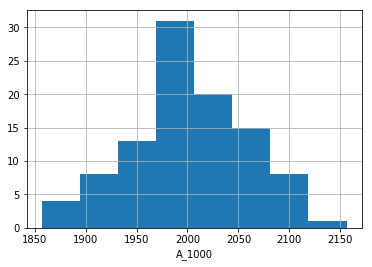
\includegraphics[width=\linewidth]{figures/task1-A.png}
  \caption{$A_{1000}$ for 100 runs}\label{fig:task1A}
\endminipage\hfill
\minipage{0.32\textwidth}
  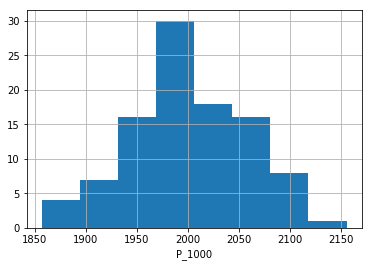
\includegraphics[width=\linewidth]{figures/task1-P.png}
  \caption{$P_{1000}$ for 100 runs}\label{fig:task1P}
\endminipage\hfill
\minipage{0.32\textwidth}%
  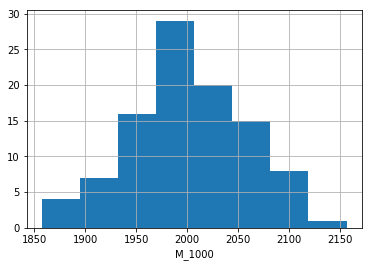
\includegraphics[width=\linewidth]{figures/task1-M.png}
  \caption{$M_{1000}$ for 100 runs}\label{fig:task1M}
\endminipage
\end{figure}


According to law of large numbers (LLN), $A_{1000}, P_{1000}, M_{1000}$ should satisfy normal distributions since each step in Lévy process can be considered as a reiterative trial, with means as:

For A,  
\begin{eqnarray*}
\mu_A& = &1000\mu_Y + 1000\mu_V - 1000\mu_W\\
&=&\frac{1000}{\lambda_2} + \frac{1000}{-\frac{\mu}{\sigma^{2}}+\sqrt{\frac{\mu^{2}}{\sigma^{4}}+\frac{2 \lambda_1}{\sigma^{2}}}} - \frac{1000}{\frac{\mu}{\sigma^{2}}+\sqrt{\frac{\mu^{2}}{\sigma^{4}}+\frac{2 \lambda_1}{\sigma^{2}}}} \\
&=&1000(1+\frac{1}{\sqrt{3}-1}-\frac{1}{\sqrt{3}+1}) = 2000
\end{eqnarray*}
It is similar to compute that 
$$\mu_P = 999\mu_Y + 1000\mu_V - 1000\mu_W = 1999$$


The 100 test results are summarized in table \ref{tab:task1}.
\begin{table}[h]
    \centering
        \caption{Mean and variance of different coordinates}
    \begin{tabular}{cccc}
    \hline
      Parameter   & Mean & Variance &Standard Deviation\\ \hline
       $A_{1000}$  & 2002.15&3312.29 & 57.84\\
       $P_{1000}$  & 2001.26 & 3324.44 & 57.95\\
       $M_{1000}$ & 2002.30 & 3313.83 & 57.86\\
       \hline
    \end{tabular}
    \label{tab:task1}
\end{table}

\newpage
\section{Algorithm Explanation}

\subsection{Original Lévy Process}
The formula below is a subclass of the Lévy process, the introduction of relevant parameters is cited from the material \cite{Brownian} below.
$$
X_{t}=\mu t+\sigma B_{t}+\sum_{i=1}^{N_{t}} Y_{i}
$$

\begin{itemize}
    \item $\mu$ is called the linear drift of the process.
    \item $\sigma$ is called the Gaussian intensity of the process.
    \item $\left\{B_{t}\right\}_{t \geq 0}$ is a standard Brownian motion (that is, a continuous-time stochastic process with independent and stationary increments and with $B_{t} \sim N(0, t)$ for all $t \geq 0$ and $B_{0}=0$).
    \item $\left\{N_{t}\right\}$ is a Poisson process of intensity $\lambda \geq 0$ with inter-arrival times $T_{1}, T_{2}, T_{3}, ...$ (recall that $T_{i} \sim E x p(\lambda)$) and arrival times $S_{1}, S_{2}, S_{3}, ...$ (recall that $S_{n} = \sum_{i=1}^{n} T_{i}$).
    \item $Y_{1}, Y_{2}, Y_{3}$ is a sequence of independent and identically distributed random variables with distribution F. 
\end{itemize}
\vspace{0.2cm}


\subsection{Discrete Skeleton}
\subsubsection{Generation of Discrete Skeleton}
Simulation of $X_{t}$ consists simulating the Brownian motion, of which process is generally difficult and inefficient. Hence, a discrete ``skeleton”\cite{Brownian} of $
\left\{X_{t}\right\}_{t \geq 0}\left(\operatorname{say}\left\{\left(P_{i}, A_{i}, M_{i}\right)\right\}_{i \in \mathbb{N}}\right.$, a 3-coordinate discrete stochastic process) is introduced to transform the simulation of continuous process to discrete one. 
\begin{itemize}
    \item $P_{i}$ is equal to $X_{S_{i}^{-}}$, that is, equal to the process $\left\{X_{t}\right\}_{t \geq 0}$ prior to its i-th jump.
    \item $A_{i}$ is equal to $X_{S_{i}}$, that is, equal to the process $\left\{X_{t}\right\}_{t \geq 0}$ after its i-th jump.
    \item $M_{i}$ is equal to $\sup _{0 \leq s \leq S_{i}} X_{s}$, that is, the maximum of $\left\{X_{t}\right\}_{t \geq 0}$ up to the time of its i-th jump.

\end{itemize}

With the discrete skeleton, one is able to describe the ${X}_t$ at the time point ${S}_i$ (i.e. the moment can be interpreted either before or after the jump.) However, the continuous process between ${X}_t$ corresponding to the Brownian motion can not be illustrated in this way.



\subsubsection{Principle of Discrete Skeleton}
1. Theorem\cite{Brownian}:
\begin{itemize}
    \item Assume $ T \sim E x p(\lambda)$.
    \item $ V=\max _{0 \leq t \leq T} \mu t+\sigma B_{t}$, where $V_{i}$ will be the highest point that $\left\{\mu t+\sigma B_{t}\right\}_{t \geq 0}$ reaches before the next inter-arrival time $T_{i}$.
    \item $W=\left(\max _{0 \leq t \leq T} \mu t+\sigma B_{t}\right)-\left(\mu T+\sigma B_{T}\right)$, where ${W}_{i}$ will be the point whose value equals to $V_{i}$ minus the value at time $T_{i}$.
    \item $V \sim E x p\left(\phi_{1}\right)$, where
    $\phi_{1}=-\frac{\mu}{\sigma^{2}}+\sqrt{\frac{\mu^{2}}{\sigma^{4}}+\frac{2 \lambda}{\sigma^{2}}}$
    \item $W \sim E x p\left(\phi_{2}\right)$, where 
    $\phi_{2}=\frac{\mu}{\sigma^{2}}+\sqrt{\frac{\mu^{2}}{\sigma^{4}}+\frac{2 \lambda}{\sigma^{2}}}$
\end{itemize}

2. Induction:
\begin{enumerate}
    \item[(1)] $T \sim E x p(\lambda)$, which means
    the linear drift and Brownian motion continuously take place during the time interval $T_{i-1}$ before the i-th jump occurring at the point $S_{i}$
    \item[(2)] $V$ and $W$ follow the exponential distribution with different rate, it is simple to simulate $V_{i}$ and $W_{i}$. Apparently, $V_{i}-W_{i} = \mu T_{i}+\sigma B_{{T}_{i}}$, then it is easy to obtain the value of the process at time $T_{i}$, which is $V_{i}-W_{i}$ (i.e. the combination of linear drift and Brownian motion during $T_{i}$);
    \item[(3)] Simulate $Y_{i}$ following the specific distribution F with corresponding parameters, where $Y_{i}$ means the size of i-th jump;
    \item[(4)] From the illustration before, the discrete ``skeleton'' of $\left\{X_{t}\right\}_{t \geq 0}$ can be expressed as:
    
    \begin{figure}[H]
    \centering
    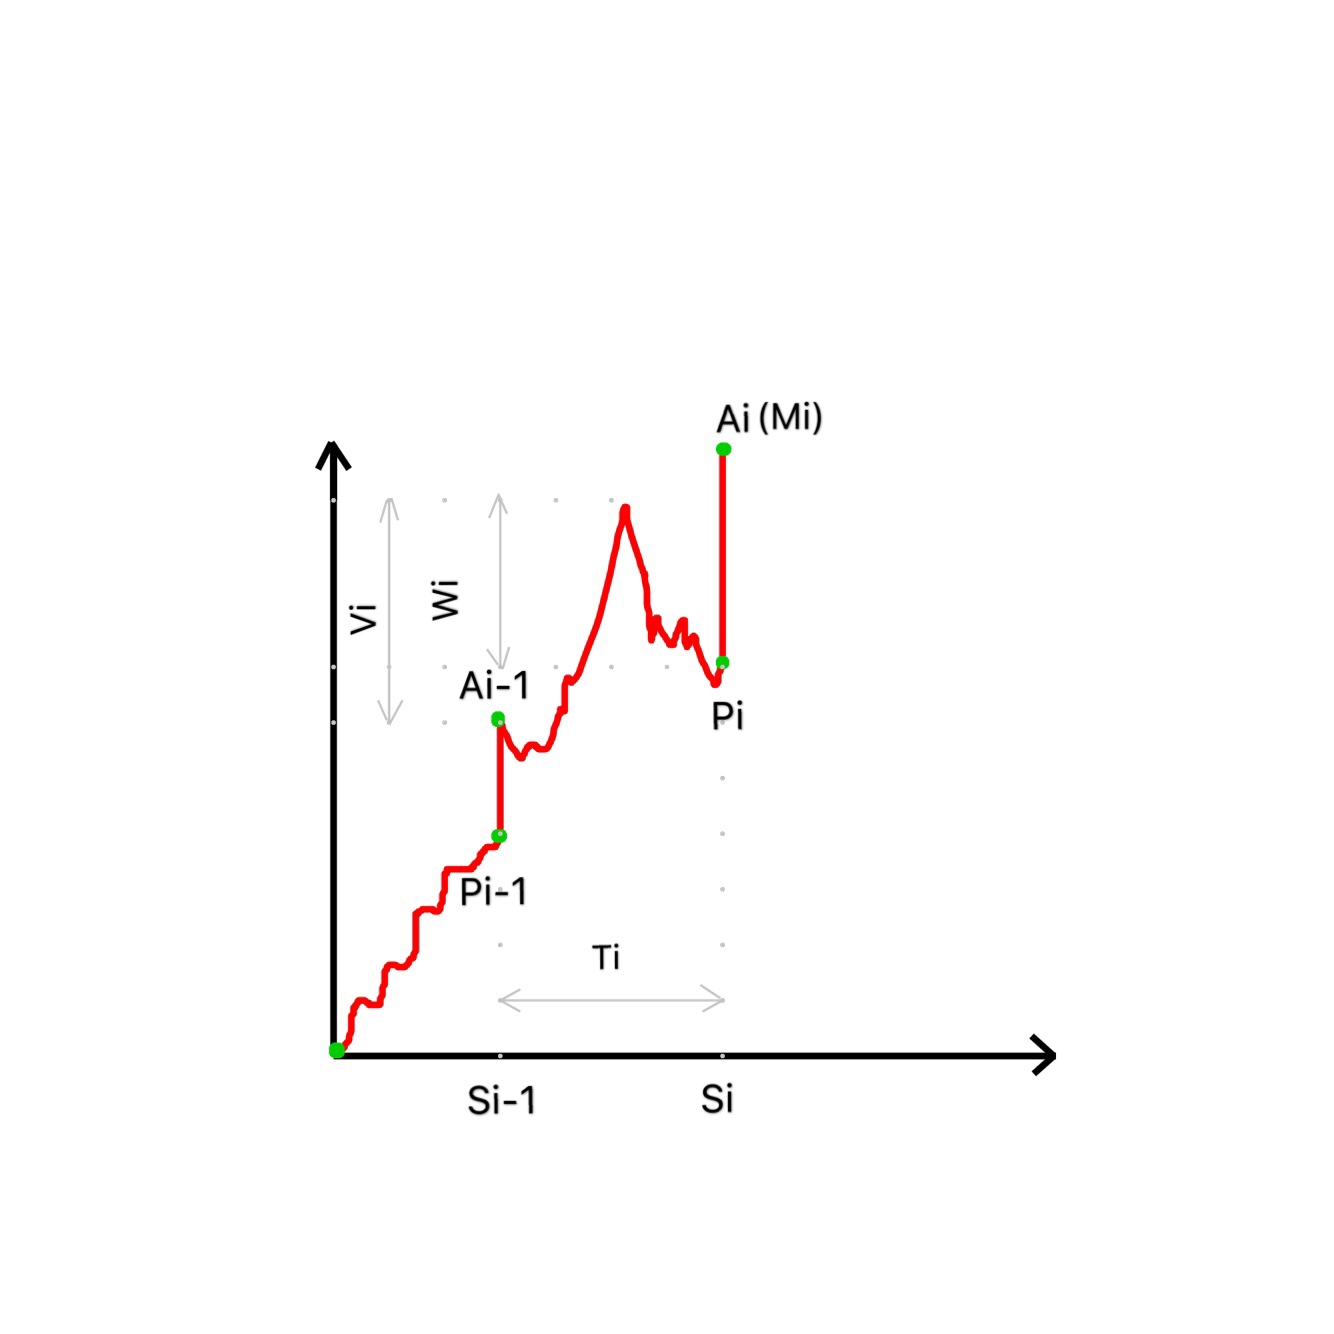
\includegraphics[scale=0.25]{figures/Illustration.png}
    \caption{Illustration}
    \label{fig:my_label}
\end{figure}
    
    \begin{itemize}
        \item $P_{i}=A_{i-1}+\left(V_{i}-W_{i}\right)$, which means $P_{i}$ equals to the sum of:\\
        a. The value of the former point $A_{i-1}$ which is obtained after (i-1)-th jump;\\
        b. The value of the process $\mu T_{i}+\sigma B_{{T}_{i}}$.
        
        \item $A_{i}=A_{i-1}+\left(V_{i}-W_{i}\right)+Y_{i}$, which means $A_{i}$ equals to $P_{i}+Y_{i}$ (i.e. the value of $P_{i}$ plus the size of i-th jump).
        
        \item $M_{i}=\max \left\{M_{i-1}, A_{i-1}+V_{i}, A_{i-1}+\left(V_{i}-W_{i}\right)+Y_{i}\right\}$, which means $M_{i}$ equals to the maximum value of all the points in time period [0, $S_i$].  
    \end{itemize}{}
    
\end{enumerate}{}







\newpage



\section{Different $\mu$, $\sigma$, $\lambda$ Verification}
The whole Lévy process $X_t$ can be treated as normal Brownian motion($X_{t}=\mu t+\sigma B_{t}$) plus a jump ($\sum_{i=1}^{N_{t}} Y_{i}$). In general, $\mu$ contributes to the linear drift and $\sigma$ is relevant to the motion variance. The jump magnitude is controlled by $Y_i$.

The jump arrival time interval $T$ is an exponential distribution with $\lambda$. The total time $S$ is accumulation of $T$ which is an Erlang distribution with parameters of jump numbers and $\lambda$. For this reason, the last jump arrival time is stochastic in each simulation.

Because $\mu$ and $\sigma$ influences normal Brownian motion only so the jump element can be excluded when investigating independent different values of $\mu$ and $\sigma$. According to the characteristics of Brownian motion, in any time $S$, the mean value of the change of $X_t$ is 
$$ E(\mu t+\sigma B_{S})=\mu S+\sigma E(B_S)$$
Because $B_S$ is standard Brownian motion subjects to normal distribution with mean is $0$, $E(B_S)=0$. So the final mean value is $\mu S$.

Regarding to variance, it can be calculated by
$$V[\mu t+\sigma B_{t}]=V[\mu S]+V[\sigma B_{S}]+2Cov[B_{S}, S]$$
where
$$V[\mu S]=\mu^2 V[S] $$
$$V[\sigma B_S]=\sigma^2(E[V(B_S|S]] + V[E[B_S|S]])= \sigma^2 E[S]$$
$$Cov[B_{S}, S]=E[S*B_S] – E[S]E[B_S] = E[S*B_S]=0$$

Remind that S follows Erlang distribution with $\lambda$ $$V[S]=\frac{Total Jump Numbers}{\lambda^2}$$
$$E[S]=\frac{Total Jump Numbers}{\lambda}$$

So the final variance
$$V[\mu t+\sigma B_{t}]=\mu^2 {\frac{Total Jump Numbers}{\lambda^2}}+ \sigma^2 {\frac{Total Jump Numbers}{\lambda}}$$

Assume that the jump $Y_i$ is an exponential distribution of $\lambda_Y=1$ in simulation. In this case it is quite obvious that the motion will reach higher if $\lambda_Y$ increases. But if the $\mu$ changes in opposite direction of $\lambda_Y$, the motion will be pull back. The detailed analysis of this is described \ref{4.4} .

\subsection{Different $\mu$}
To verify how $\mu$ influences the motion, we like to keep the $\sigma$ and $\lambda$ as constant, in simulation both $\sigma$ and $\lambda$ are set to 1.

In the case of $\mu>0$ the path slope goes up as $\mu$ increases and vice verse. When the $\mu$ is extreme small($10^{-5}$) the path is similar to the Brownian motion without linear drift but the motion path is dominated by linear drift if $\mu$ is very large ($10^{5}$). The simulation result is shown on Figure \ref{fig:diffmu}

Consider the case $\mu=10^{5}$, the simulation generates 100 $A_{1000}$ at time $S_{1000}$ (since each run the last arrival time is scholastic so $S_{1000}$ is calculated as a mean of 100 last arrival time). The result of mean of 100 $A_{1000}$ is $1.0001\times 10^8$ and the theoretical calculation $\mu S_{1000}$ is $9.9926\times 10^7$, they are nearly the same.

When the $\mu=10^{-5}$, it is close to 0, the motion variance becomes very large because there is almost no linear drift. The theoretical mean value of $A_{1000}$ in 100 runs is $0.01$ but the actual mean of $A_{1000}$ is approximate -1.12, this is since the sample is only 100 and if it is increased to 100000, the mean of $A_{1000}$ is $0.018$ is improved to very close to the theoretical value.

Apparently if $\mu<0$ the motion will move to the negative $y$ axles and the slope reduces as $\mu$ decreases.  

\begin{figure}[H]
    \centering
    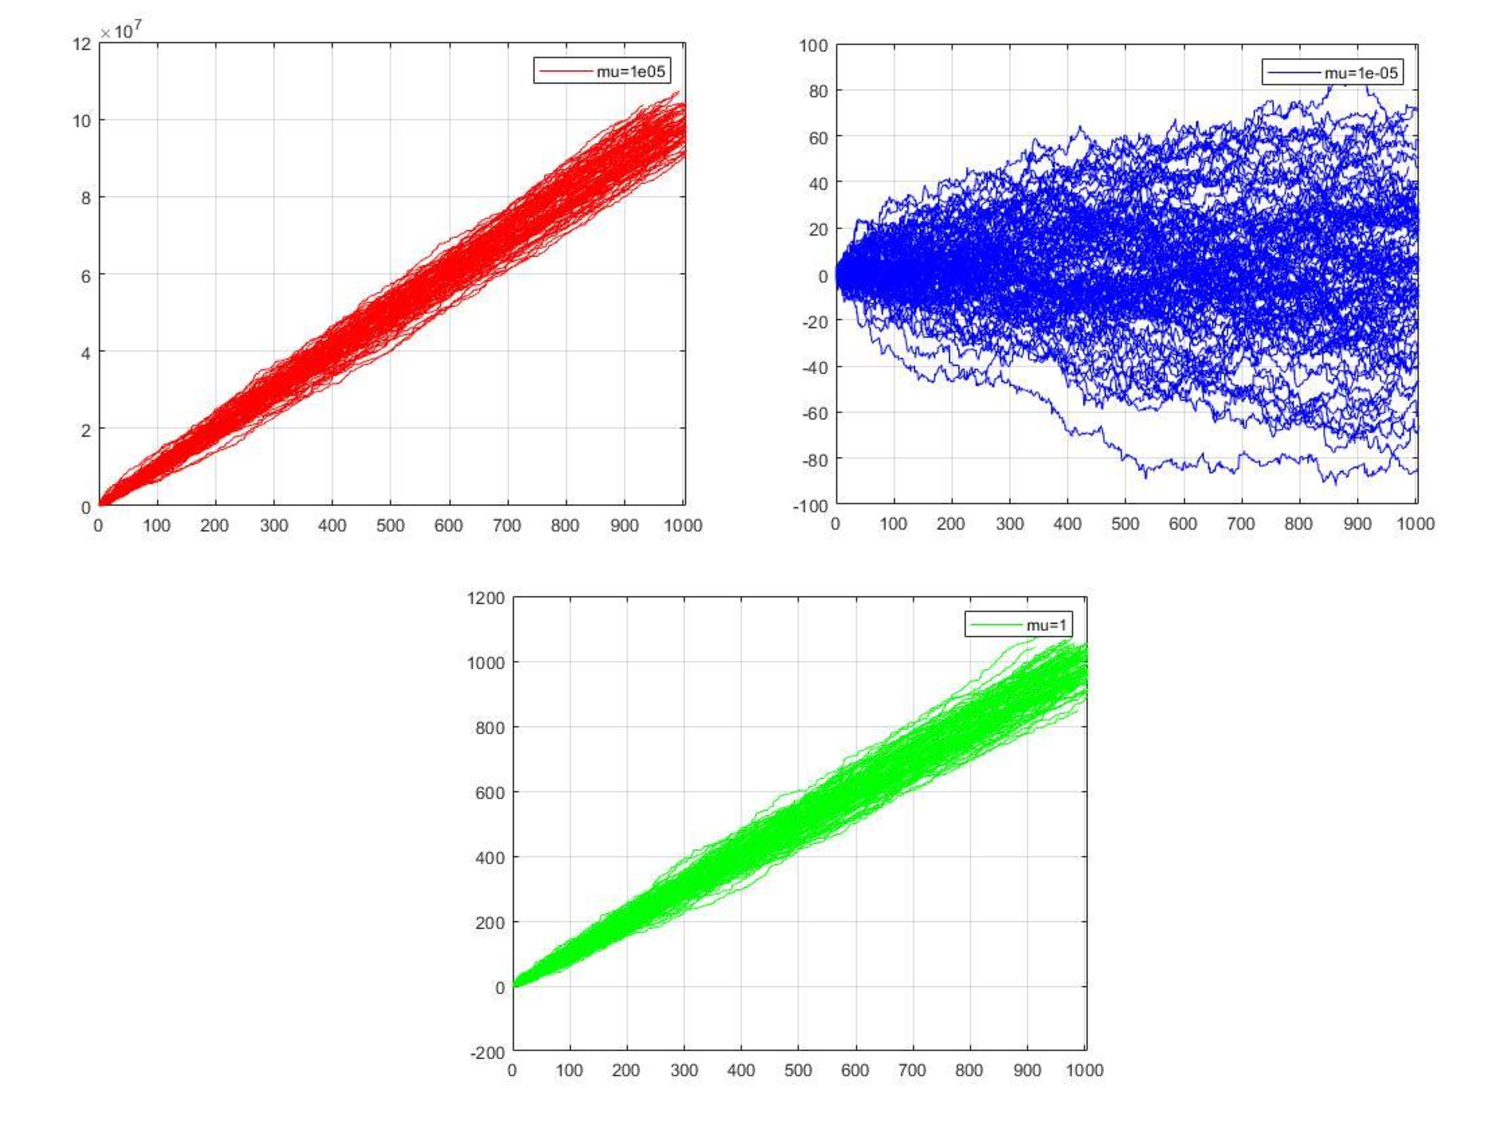
\includegraphics[scale=0.65]{figures/Task3/Diff_mu.pdf}
    \caption{Path with different $\mu$}
    \label{fig:diffmu}
\end{figure}

\subsection{Different $\sigma$}
Similarly, to verify $\sigma$, both $\mu$ and $\lambda$ are set to $1$.

$\sigma$ determines the variance for $X_t$. When $\sigma=10^{5}$, as shown on Figure \ref{fig:diffsigma}, the variance become very large as $\sigma$ is large. Consider a 100 loops simulation the variance among $A_{1000}$ is $9.982\times 10^{12}$ which is quite close to theoretical value ($1.0\times 10^{13}$)

If $\sigma$ becomes extreme small, $10^{-5}$, the motion again control by the linear drift and the variance of end values is $1.109\times 10^{3}$ and the theoretical result is $1.0\times 10^{3}$. 
\begin{figure}[H]
    \centering
    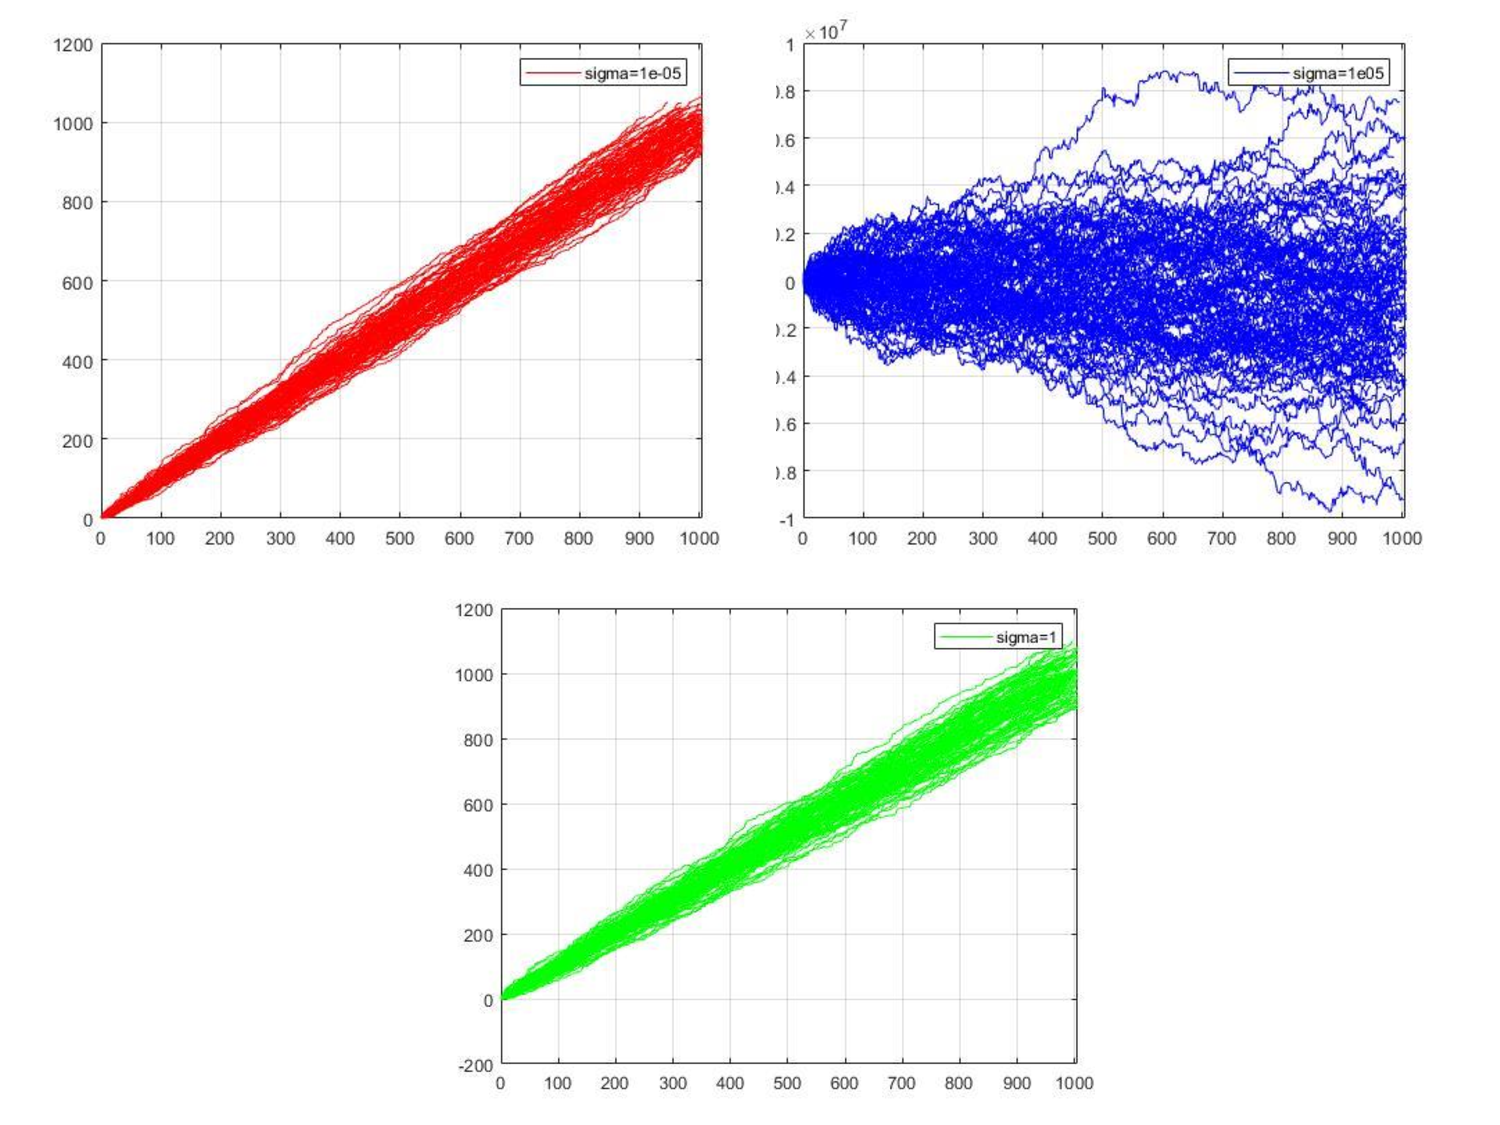
\includegraphics[scale=0.65]{figures/Task3/Diff_sigma.pdf}
    \caption{Path with different $\sigma$}
    \label{fig:diffsigma}
\end{figure}

\subsection{Different $\lambda$}
The $\lambda$ determines the time interval of $T$ and the total time $S$ that is Erlang distribution. If $\lambda$ is very large ($10^{5}$), both $T$ and $S$ are very small that indicates movement are basic only from origin to y-axle, as Figure \ref{fig:difflambda} shows. But when the $\lambda$ is set to $10^{-5}$, $T$ and $S$ are quite large which specifies it takes much more time to finish the entire path motion.
\begin{figure}[H]
    \centering
    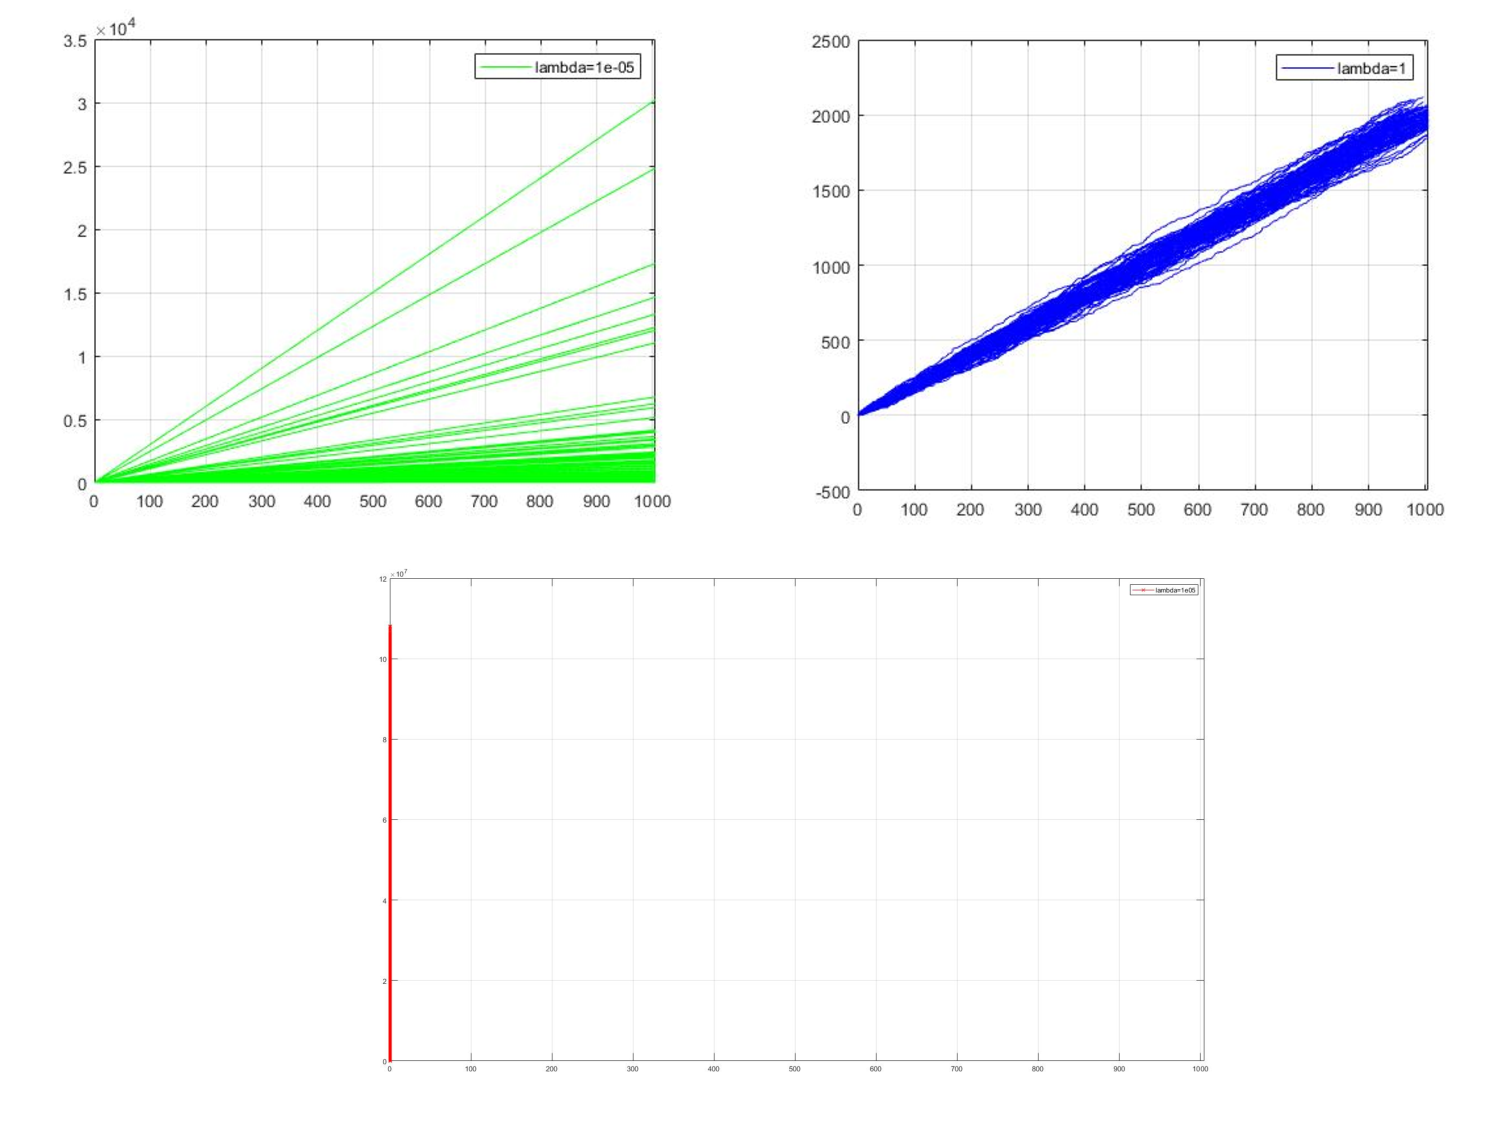
\includegraphics[scale=0.65]{figures/Task3/Diff_lambda.pdf}
    \caption{Path motion with different $\lambda$  }
    \label{fig:difflambda}
\end{figure}

\subsection{$\mu$ vs. $\lambda_Y$} \label{4.4}
Take the jump into consideration, in the situation of $\mu=-1$ and $\lambda_Y=1$, it indicates the linear drift can be counteracted by the jump, then the path becomes like the case of $\mu$ is pretty small, the Brownian motion without linear drift. 
\begin{figure}[H]
    \centering
    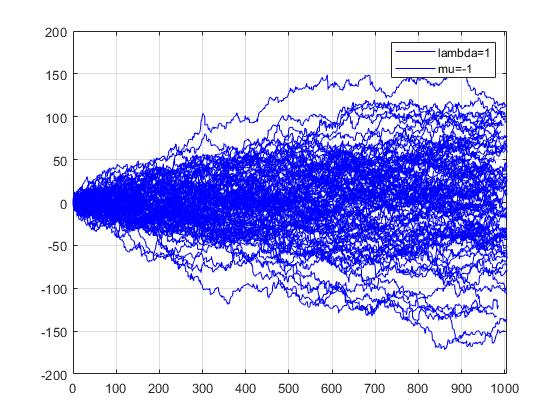
\includegraphics[scale=0.6]{figures/Task3/lambda=1mu=-1.jpg}
    \caption{Simulation result with $\mu=-1$ and $\lambda_Y=1$}
    \label{fig:my_label}
\end{figure}

%\subsubsection{$\mu$ vs. $\sigma$}
%In the case of 









\newpage
\section{Experimentation $Y_i$ with different distribution}

As $Y_i$ corresponds to the length of each jump, it is worth analyzing various distributions of $Y_i$ to describe $\left\{X_{t}\right\}_{t \geq 0}$ better.

Four types of distributions are experimented in this case, i.e. Exponential distribution, Erlang distribution, Hyper-exponential distribution and Pareto distribution.
Setting the mean value of each distribution to be 1, the variances are different shown as below. 

\begin{figure}[H]
    \centering
    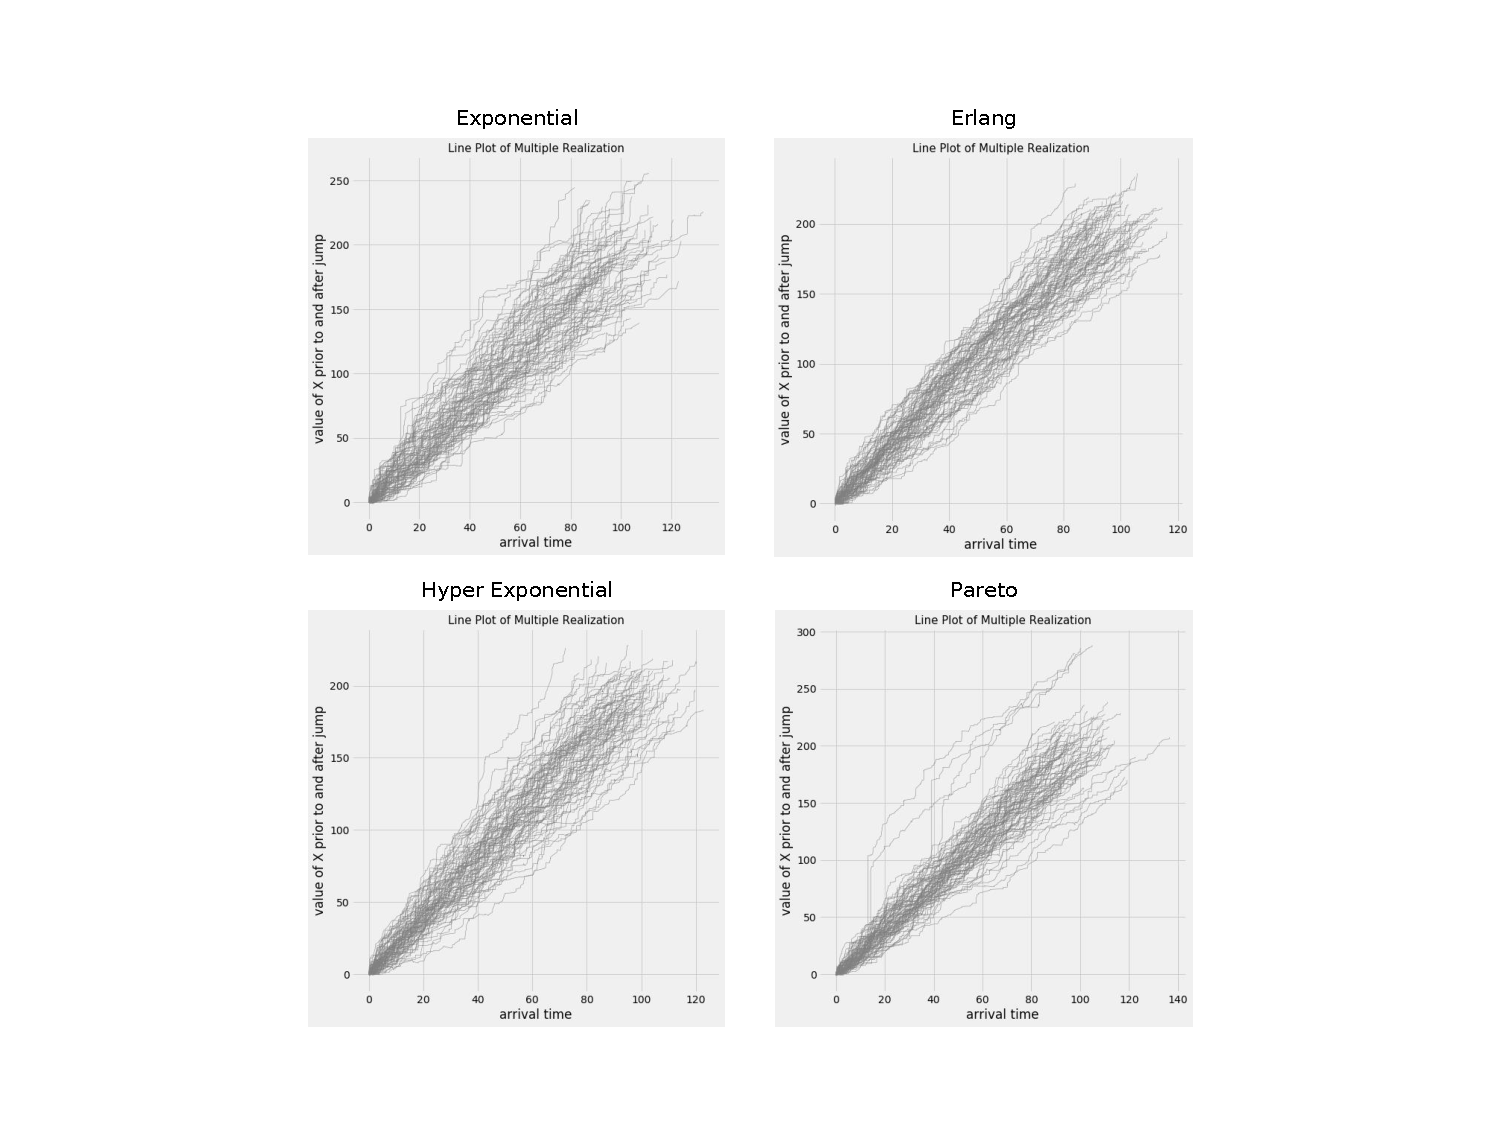
\includegraphics[scale = 0.9]{figures/task4.pdf}
    \caption{$Y_{i}$ following different $F$ distributions($\mu = 1$, $N_{jump} = 100$)}
    \label{fig:task4}
\end{figure}

\begin{itemize}
    \item Erlang distribution presents the lowest variance of path.
    \item Hyper-exponential distribution gives higher variance than the Exponential distribution.
    \item Pareto distribution often results in a higher probability of extreme observations, leading to large variance as well. Therefore, some paths on the bottom-right of figure \ref{fig:task4} have much longer jump at certain steps.
\end{itemize}

In order to examine the simulate value, the theoretical variance are calculated here:
\begin{enumerate}
    \item[(1)] Erlang distribution(k = 2):\\
    Combine two independent exponential variables with mean $\frac{1}{\lambda}$ each, then the variance is:\\
    $\mathbb{V}(X)=\frac{n}{\lambda^{2}} = \frac{2}{2^{2}} = \frac{1}{2}$
    
    \item[(2)] Exponential distribution:\\
    $\mathbb{V}(X)=\frac{1}{\lambda^{2}} = \frac{1}{1^2} = 1$ 
    
    \item[(3)] Hyper-exponential distribution:\\
    $\mathbb{V}(X) = \left[\sum_{i=1}^{n} \frac{p_{i}}{\lambda_{i}}\right]^{2}+\sum_{i=1}^{n} \sum_{j=1}^{n} p_{i} p_{j}\left(\frac{1}{\lambda_{i}}-\frac{1}{\lambda_{j}}\right)^{2}
    = 5.5$
    
    \item[(4)] Pareto distribution(k = 2):\\
    Because k is set to 2, then the variance of Pareto is infinite.
    
    
    
\end{enumerate}

Hence, the simulation accords with expected result of theory.









\newpage
\section{Estimation of Probability Upcrossing level $a$}
Connecting the Levy process with real-world case, one could take the change of stock price as an instance. The stock price probably fluctuates around the opening price instead of always surpassing or falling below. In our case, the linear drift of $\left\{X_{t}\right\}_{t \geq 0}$ given by $\mu T$ shall offset the effect of jumps in the long run. What is more concerning is that which coordinate of the discrete skeleton $\left\{\left(P_{i}, A_{i}, M_{i}\right)\right\}_{i \in \mathbb{N}}$ is more relevant to evaluate. The value of $M_i$ always records the highest level which $\left\{X_{t}\right\}_{t \geq 0}$ have ever reached before the $i^{th}$ jump. Then, for a path with $i$ jumps, if $M_i$ does not upcross level $a$, the path can never surpass level $a$.

\\
Figure \ref{fig:task5-3} shows 100 paths of simulated Lévy process. The mean of $Y_i$ for each path is set to be 1 and the drift factor $\mu$ to be -1. For the given value of $a$, the probability of $\left\{X_{t}\right\}_{t \geq 0}$ upcrossing level $a$ is calculated as the frequency of the exceeding paths over total simulated paths. Remind that, in this case, $\sigma$ is assigned to be 1 which leads to $\sigma B_t$ being a standard Brownian Motion. Thus, the probability of upcrossing is more likely to be determined by the variance of $(V_i-W_i)$ and $\sum_1^{N_t}Y_i$.
\begin{figure}[H]
    \centering
    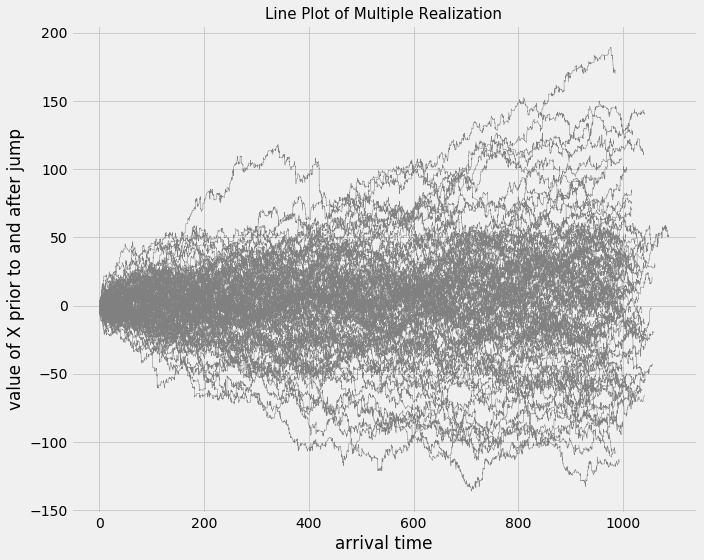
\includegraphics[scale = 0.45]{figures/task5-3.png}
    \caption{Simulation with $Y_i \sim {exp(\lambda = 1)}$, $\mu = -1$, $N_{jump} = 1000$, $\sigma$ = 1}
    \label{fig:task5-3}
\end{figure}

Figure \ref{fig:task5-4} illustrates the probability given different $a$-value. Considering $Y_i$ following the  exponential distribution, when the value of $a$ increases, the probability of $\left\{X_{t}\right\}_{t \geq 0}$ surpassing the given value decreases from 100\% to 0\%. If the level $a$ is set to be above 200, it almost never reaches within 1000 jumps. Meanwhile, considering all four different distributions of $Y_i$, the probability of upcrossing level $a$ conforms to the result of figure \ref{fig:task4} which mainly related to the variance of each distribution.

\begin{figure}[H]
    \centering
    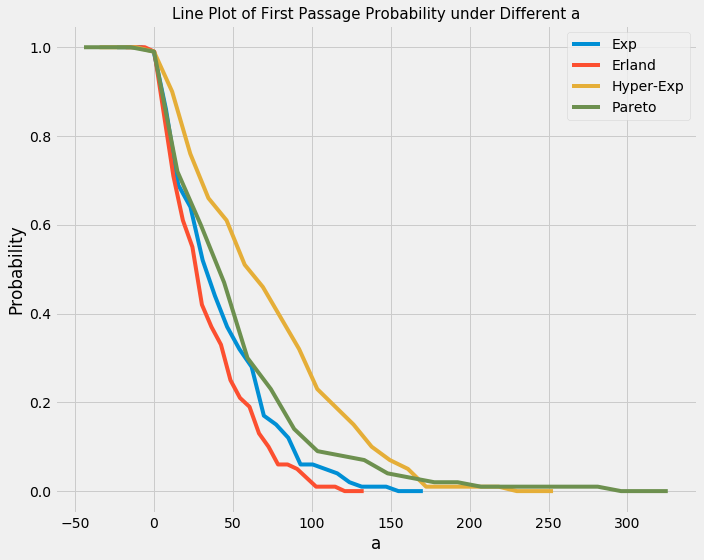
\includegraphics[scale = 0.45]{figures/task5-4.png}
    \caption{Fist passage probability of different distribution functions under different $a$ values}
    \label{fig:task5-4}
\end{figure}


\newpage





% \\section{References}

\bibliographystyle{unsrt}
\bibliography{bibtex/bibliography}


\section{Appendix}

Following packages and functions are used in this project.

\begin{Shaded}
\begin{Highlighting}[]
\CommentTok{## basic packages}
\KeywordTok{library}\NormalTok{(knitr)}
\KeywordTok{library}\NormalTok{(kableExtra)}
\KeywordTok{library}\NormalTok{(tidyverse)}
\KeywordTok{library}\NormalTok{(conflicted)}
\KeywordTok{library}\NormalTok{(magrittr)}
\KeywordTok{library}\NormalTok{(broom)}
\CommentTok{# library(car)}
\CommentTok{## paticular packages for this project}
\KeywordTok{library}\NormalTok{(lmtest)}
\KeywordTok{library}\NormalTok{(corrr)}
\KeywordTok{library}\NormalTok{(tseries)}
\KeywordTok{library}\NormalTok{(corrplot)}
\KeywordTok{source}\NormalTok{(}\StringTok{"./funcs.R"}\NormalTok{)}
\end{Highlighting}
\end{Shaded}

The data set is defined as follows based on file \texttt{recs.csv}:

\begin{Shaded}
\begin{Highlighting}[]
\KeywordTok{set.seed}\NormalTok{(}\DecValTok{6}\NormalTok{)}
\NormalTok{dat <-}\StringTok{ }
\StringTok{  }\KeywordTok{read_csv}\NormalTok{(}\StringTok{"./data/recs.csv"}\NormalTok{) }\OperatorTok
\StringTok{  }\NormalTok{dplyr}\OperatorTok{::}\KeywordTok{slice}\NormalTok{(}\KeywordTok{sample}\NormalTok{(}\KeywordTok{nrow}\NormalTok{(.), }\DecValTok{300}\NormalTok{)) }\OperatorTok
\StringTok{  }\KeywordTok{mutate}\NormalTok{(}\DataTypeTok{y =} \KeywordTok{log}\NormalTok{(KWH }\OperatorTok{/}\StringTok{ }\NormalTok{NHSLDMEM)) }\OperatorTok
\StringTok{  }\KeywordTok{mutate}\NormalTok{(}\DataTypeTok{x8 =}\NormalTok{ TOTROOMS }\OperatorTok{+}\StringTok{ }\NormalTok{NCOMBATH }\OperatorTok{+}\StringTok{ }\NormalTok{NHAFBATH) }\OperatorTok
\StringTok{  }\NormalTok{dplyr}\OperatorTok{::}\KeywordTok{select}\NormalTok{(y, }\DataTypeTok{x2 =}\NormalTok{ NHSLDMEM, }\DataTypeTok{x3 =}\NormalTok{ EDUCATION, }\DataTypeTok{x4 =}\NormalTok{ MONEYPY, }\DataTypeTok{x5 =}\NormalTok{ HHSEX, }
    \DataTypeTok{x6 =}\NormalTok{ HHAGE, }\DataTypeTok{x7 =}\NormalTok{ ATHOME, x8) }\OperatorTok
\StringTok{  }\KeywordTok{mutate_at}\NormalTok{(}\KeywordTok{seq}\NormalTok{(}\DecValTok{2}\NormalTok{, }\DecValTok{8}\NormalTok{), as.integer) }\OperatorTok\StringTok{  }\CommentTok{# make continuous variables discrete}
\StringTok{  }\KeywordTok{mutate}\NormalTok{(}\DataTypeTok{x5 =} \OperatorTok{-}\StringTok{ }\NormalTok{x5 }\OperatorTok{+}\StringTok{ }\DecValTok{2}\NormalTok{) }
\end{Highlighting}
\end{Shaded}

\hypertarget{introduction}{%
\subsection{Introduction}\label{introduction}}

Different variables are summarized in the following table. \texttt{y},
the logarithm of averaged electricity consumption, is the variable that
we are interested in. Specifically, The electricity consumption refers
to the electricity usage of the house/studio where the respondent lives
in 2015, measured in kilowatthours. The quantity is average by the
number of household members in the house/studio. That way, it roughly
represent the level of electricity consumption of the respondent. Other
variables are discussion in the following table.

\begin{longtable}[]{@{}lll@{}}
\toprule
Sym & Abbr & Definition\tabularnewline
\midrule
\endhead
z & KWH & electricity consumption\tabularnewline
y & LKWH.pers & logarithm of KWH/NHSLDMEM\tabularnewline
x2 & NHSLDMEM & number of household members\tabularnewline
x3 & EDUCATION & highest education completed\tabularnewline
x4 & MONEYPY & annual gross household income last year\tabularnewline
x5 & HHSEX & gender\tabularnewline
x6 & HHAGE & age\tabularnewline
x7 & ATHOME & number of weekdays someone is at home\tabularnewline
x8 & TOTROOMS + & number of rooms (including bathrooms)\tabularnewline
\bottomrule
\end{longtable}

Note that \texttt{x8} is a variable indicating the number of rooms of
the house/studio of the respondent. It equals the summation of
\texttt{TOTROOMS}, \texttt{NCOMBATH} and \texttt{NHAFBATH} in the
original data set. \texttt{x8} is not included in the initial analysis
(sections 1 to 7).

\texttt{x3}, the education level of the respondent, is considered as a
continuous variable in this project for simplicity. The detailed
definition of different levels is shown in the following table.

\begin{longtable}[]{@{}ll@{}}
\toprule
Level & Definition\tabularnewline
\midrule
\endhead
1 & Less than high school diploma or GED\tabularnewline
2 & High school diploma or GED\tabularnewline
3 & Some college or Associate's degree\tabularnewline
4 & Bachelor's degree (for example: BA, BS)\tabularnewline
5 & Master's, Professional, or Doctorate degree\tabularnewline
\bottomrule
\end{longtable}

The first 5 rows of the data set used can be visualized:

\begin{table}[H]
\centering
\begin{tabular}{llllllll}
\toprule
y & x2 & x3 & x4 & x5 & x6 & x7 & x8\\
\midrule
7.5 & 5 & 3 & 8 & 1 & 39 & 5 & 15\\
8.2 & 1 & 2 & 2 & 0 & 85 & 5 & 14\\
8.7 & 3 & 1 & 1 & 0 & 71 & 5 & 8\\
7.8 & 4 & 3 & 5 & 1 & 39 & 5 & 8\\
9.8 & 1 & 3 & 3 & 0 & 57 & 0 & 10\\
\bottomrule
\end{tabular}
\end{table}

In this project, we want to develop a model associating the continuous
variable, average electricity consumption, with other variables. We will
start by visualizing correlations between variables. In particular, the
two variables \texttt{x2} and \texttt{x6}, which highly correlate with
\texttt{y} will be explored. The model regressing \texttt{y} on
\texttt{x2} will be discussed in section 2. Four assumptions will be
made, three of which will be tested in section 3-5 by Jarque-Bera test
(normality), White's test (homoskedasticity) and RESET test (functional
form) respectively. According the test results and discussion in section
6, data point \texttt{36} is excluded. Then, in section 7, more
regressors are introduced and three new models are established. The
detail regarding how regressors interact with each other, namely
causality, is discussed in section 8. Based on the understanding of the
underlying mechanism, a nonlinear term and \texttt{x8} are included as
new regressors. Two new models are estimated, based on the only model
passing all tests in section 7. Finally, the model called
\texttt{mods{[}{[}7{]}{]}} is chosen as the final for presentation and
it is interpreted in section 10.

\hypertarget{data-visualization}{%
\subsection{Data Visualization}\label{data-visualization}}

It can be seen that \texttt{y} is highly correlated to \texttt{x2} and
\texttt{x6} according to the following table.

\begin{table}[H]
\centering
\begin{tabular}{lll}
\toprule
x & y & r\\
\midrule
x2 & y & -0.511\\
x3 & y & 0.034\\
x4 & y & 0.041\\
x5 & y & -0.043\\
x6 & y & 0.353\\
x7 & y & 0.040\\
x8 & y & 0.213\\
\bottomrule
\end{tabular}
\end{table}

It can be seen from the following covariance matrix that \texttt{y} is
highly correlated to \texttt{x2}, \texttt{x6} and \texttt{x8}. Besides,
\texttt{x3}-\texttt{x4}, \texttt{x2}-\texttt{x6},
\texttt{x4}-\texttt{x8} are high correlated, which will be discussed in
section 9.

\begin{center}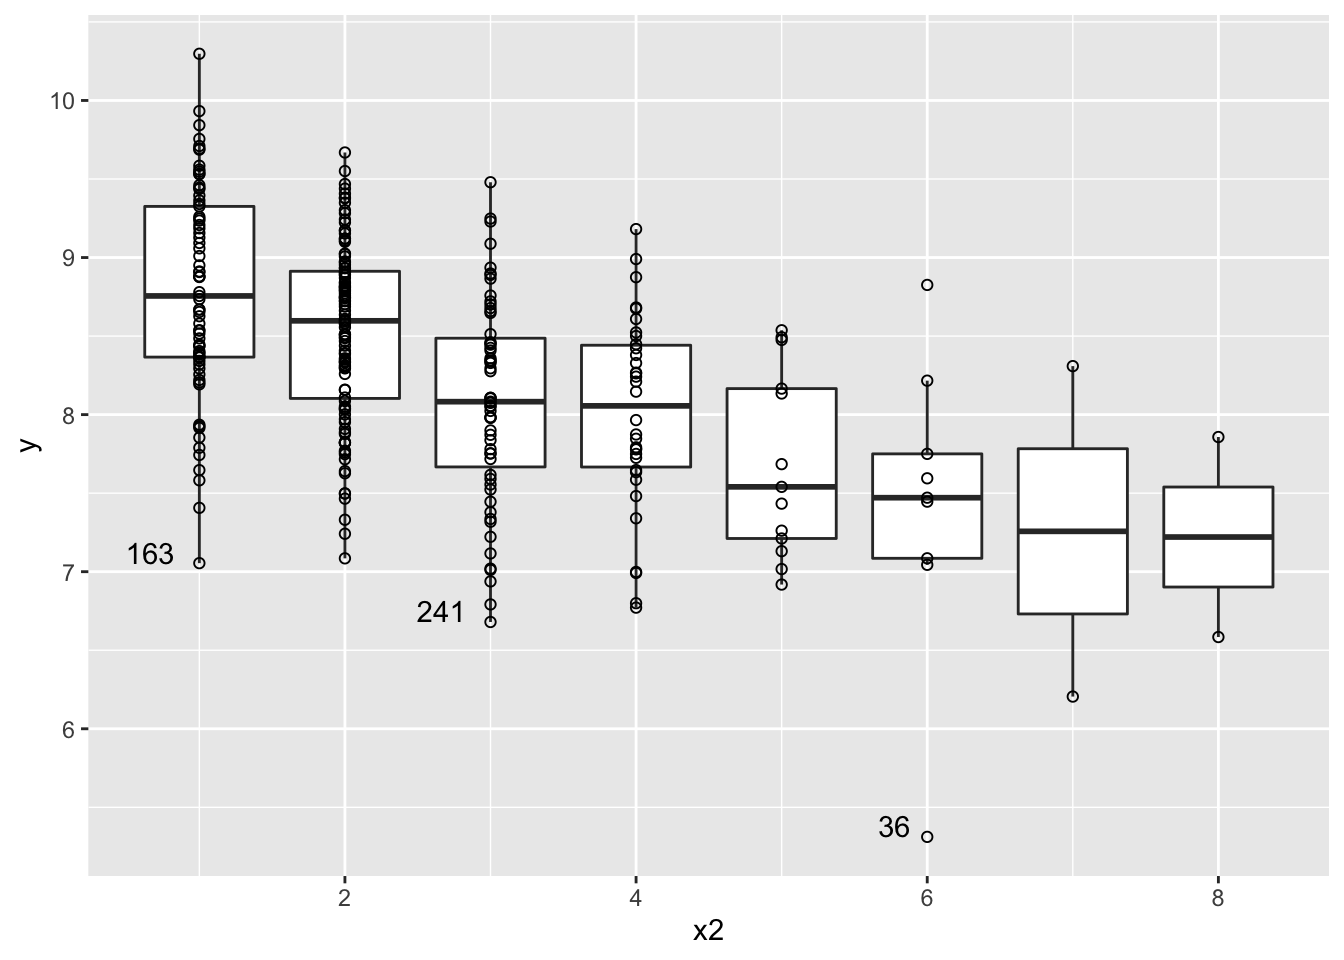
\includegraphics[width=0.48\textwidth]{main_files/figure-latex/unnamed-chunk-7-1} \end{center}

For each level of \texttt{x2} a box indicating three quantiles (25\%,
50\%, 75\%) of \texttt{y} is given. It shows that there is a tendency
for \texttt{y} to decrease with \texttt{x2} by looking at the median.
The sizes of different boxes seem to vary with different values of
\texttt{x2}. Besides, there are many observations when \texttt{x2} is
small. But it is assumed for now that the conditional variance is
constant, which will be tested section 4. Three data points with extreme
values \texttt{36}, \texttt{241} and \texttt{163} is discussed in
sections 3 and 5.

\begin{center}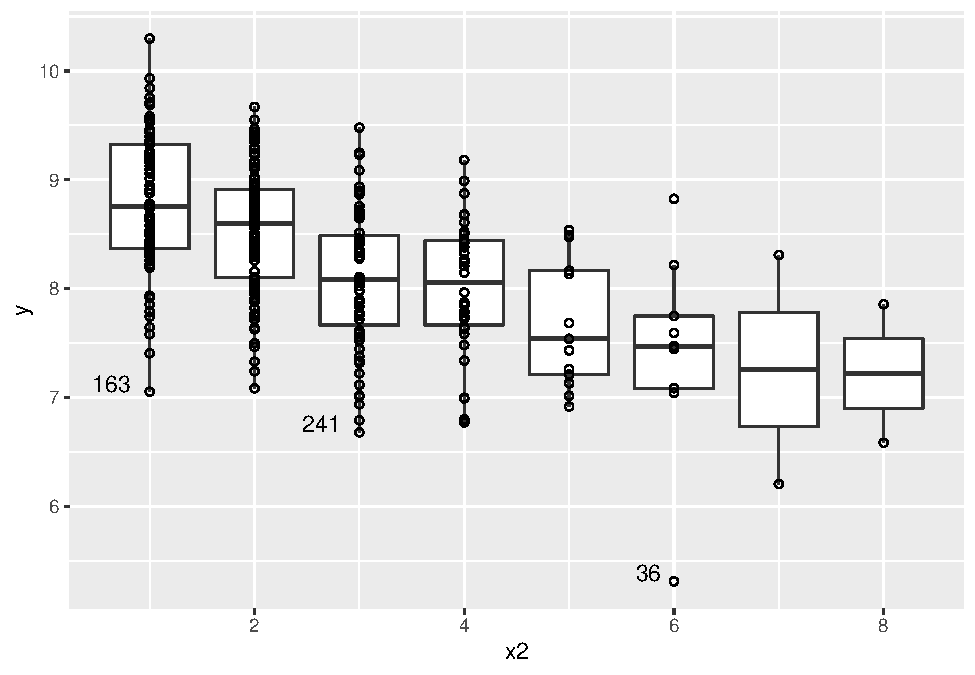
\includegraphics[width=0.48\textwidth]{main_files/figure-latex/unnamed-chunk-8-1} \end{center}

The box plot of \texttt{y} by \texttt{x6} is given. It can be seen that
the tendency is not strictly linear and the condition variance is not
stable. So we will regress \texttt{y} on \texttt{x2} first and use
\texttt{x6} as the second regressor in section 6.

\begin{center}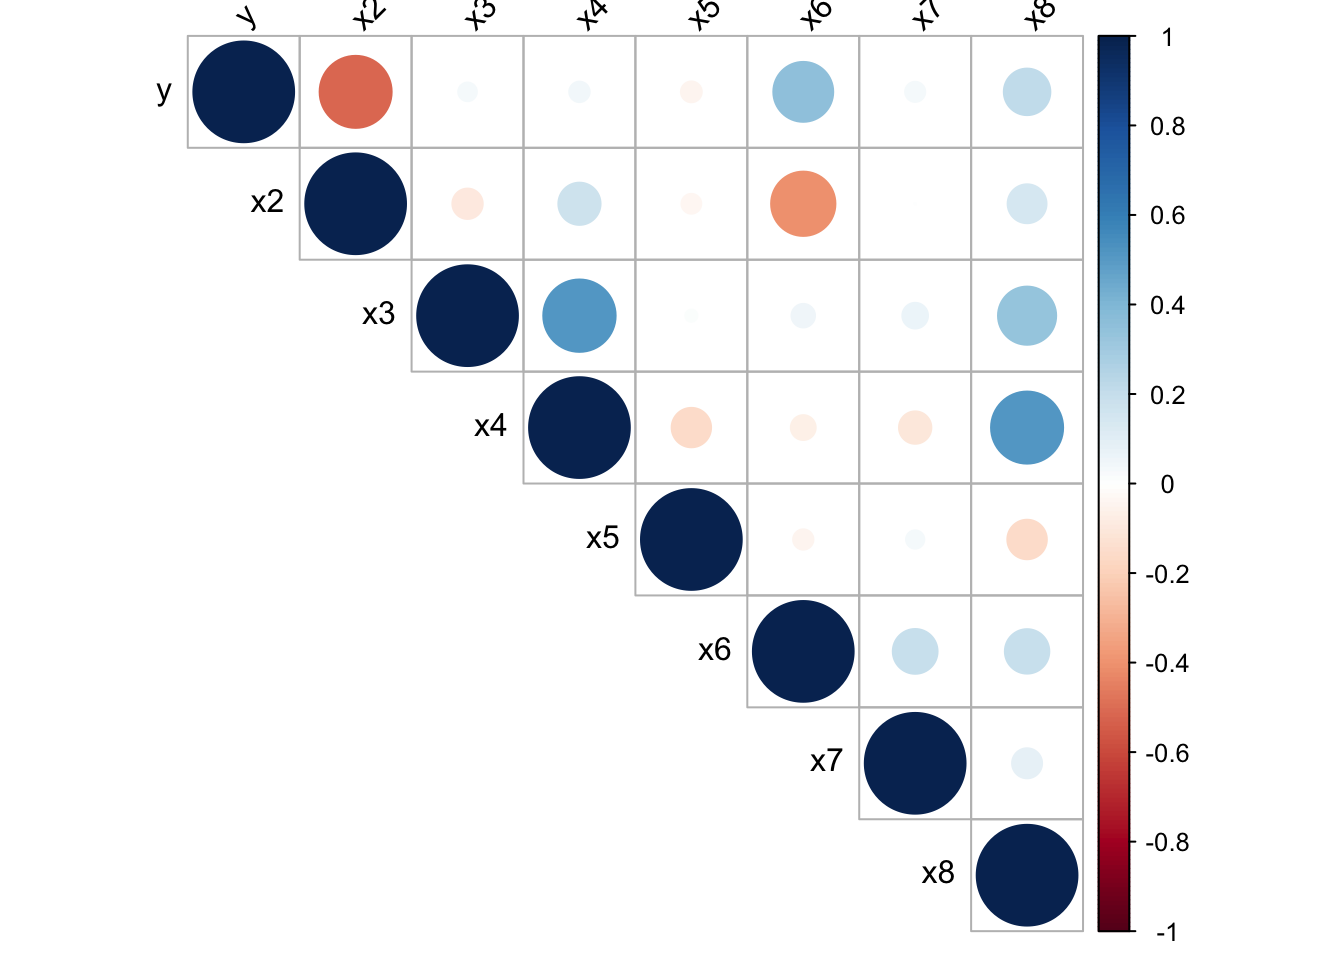
\includegraphics[width=0.48\textwidth]{main_files/figure-latex/unnamed-chunk-9-1} \end{center}

\hypertarget{regress-y-on-x2-assumptions-and-orthogonalization}{%
\subsection{\texorpdfstring{2. Regress \texttt{y} on \texttt{x2},
Assumptions and
Orthogonalization}{2. Regress y on x2, Assumptions and Orthogonalization}}\label{regress-y-on-x2-assumptions-and-orthogonalization}}

\texttt{mods{[}{[}1{]}{]}} is obtained by regressing \texttt{y} on
\texttt{x2}.

\begin{verbatim}
#> lm(formula = y ~ x2, data = dat)
\end{verbatim}

\begin{table}[H]
\centering
\begin{tabular}{lllll}
\toprule
term & estimate & std.error & statistic & p.value\\
\midrule
(Intercept) & 9.04 & 0.075 & 120 & 2.2e-254\\
x2 & -0.27 & 0.026 & -10 & 2.4e-21\\
\bottomrule
\end{tabular}
\end{table}

\begin{table}[H]
\centering
\begin{tabular}{lllllllllll}
\toprule
r.squared & adj.r.squared & sigma & statistic & p.value & df & logLik & AIC & BIC & deviance & df.residual\\
\midrule
0.26 & 0.26 & 0.63 & 105 & 2.4e-21 & 2 & -286 & 579 & 590 & 119 & 298\\
\bottomrule
\end{tabular}
\end{table}

By orthogonalizing \texttt{x2} with respect to constant 1. the following
reparameterized model can be obtained.

\begin{Shaded}
\begin{Highlighting}[]
\NormalTok{mods[[}\DecValTok{2}\NormalTok{]] <-}\StringTok{ }
\StringTok{  }\NormalTok{dat }\OperatorTok
\StringTok{  }\KeywordTok{mutate}\NormalTok{(}\DataTypeTok{x1 =} \DecValTok{1}\NormalTok{, }\DataTypeTok{x21 =}\NormalTok{ x2 }\OperatorTok{-}\StringTok{ }\KeywordTok{mean}\NormalTok{(.}\OperatorTok{$}\NormalTok{x2)) }\OperatorTok
\StringTok{  }\NormalTok{dplyr}\OperatorTok{::}\KeywordTok{select}\NormalTok{(y, x1, x21) }\OperatorTok
\StringTok{  }\NormalTok{\{}\KeywordTok{lm}\NormalTok{(y }\OperatorTok{~}\StringTok{ }\NormalTok{x1 }\OperatorTok{+}\StringTok{ }\NormalTok{x21, }\DataTypeTok{data =}\NormalTok{ .)\}}
\end{Highlighting}
\end{Shaded}

\begin{verbatim}
#> lm(formula = y ~ x1 + x21, data = .)
\end{verbatim}

\begin{table}[H]
\centering
\begin{tabular}{lllll}
\toprule
term & estimate & std.error & statistic & p.value\\
\midrule
(Intercept) & 8.36 & 0.036 & 230 & 0.0e+00\\
x21 & -0.27 & 0.026 & -10 & 2.4e-21\\
\bottomrule
\end{tabular}
\end{table}

\begin{table}[H]
\centering
\begin{tabular}{lllllllllll}
\toprule
r.squared & adj.r.squared & sigma & statistic & p.value & df & logLik & AIC & BIC & deviance & df.residual\\
\midrule
0.26 & 0.26 & 0.63 & 105 & 2.4e-21 & 2 & -286 & 579 & 590 & 119 & 298\\
\bottomrule
\end{tabular}
\end{table}

The estimated regression coefficient for \texttt{x2} in
\texttt{mods{[}{[}1{]}{]}} equals that for \texttt{x21} in
\texttt{mods{[}{[}2{]}{]}}. That is, slopes in these two models are the
same. The standard error of the intercept is reduced by 51.60 \%.

\end{document}



